\section{Quick Sort} \label{cap:2:section:qsort}

\subsection{Introdução}

O \textit{Quick} Sort é um algoritmo de ordenação bastante eficiente, seu funcionamento é baseado
na estratégia de ordenação de dividir para conquistar. Basicamente, o processo é particionar um vetor
de forma recursiva enquanto realiza a ordenação nele, utilizando uma lógica de pivot e marcador para
troca.

\subsection{Implementação}

Para o algoritmo de ordenação por particionamento, o pseudo-código utilizado para desenvolver o
algoritmo pode ser observado em \ref{quickSortP} retirado do livro \cite{cormen2022algorithms}.

\begin{pseudocode}[caption={Algoritmo de ordenação por particionamento}, label={quickSortP}]
QUICK-SORT(A, p, r)
if p < r then
    q = PARTITION(A, p, r)
    QUICK-SORT(A, p, q - 1)
    QUICK-SORT(A, q + 1, r)
\end{pseudocode}

Esse pseudo-código foi implementado na linguagem de programação C 
e pode ser observado no código seguinte:

\begin{lstlisting}[style=CStyle]
int partition(int * v, int s, int e)
{

    int pivot = v[s];

    int i = s - 1;
    int j = e + 1;

    while (1)
    {
        do
        {
            i += 1;
        } while (v[i] < pivot);

        do
        {
            j -= 1;
        } while (v[j] > pivot);
        
        if (i >= j)
        {
            return j;
        }

        swap(&v[i], &v[j]);
    }
}

void qSort(int * v, int s, int e)
{
    if (s >= 0 && e >= 0 && s < e)
    {
        int p = partition(v, s, e);
        qSort(v, s, p);
        qSort(v, p + 1, e);
    }
}
\end{lstlisting}

\subsection{Análise do algoritmo e notação assintótica}

Para que seja determinada a razão de crescimento do algoritmo de ordenação por particionamento, é necessário
perceber os tempos de execução de cada linha do pseudo-código \ref{quickSortP}.
Nesse caso, pode-se ter como base a equação \ref{cap:2:eq:quickSort:1}.

\begin{equation} \label{cap:2:eq:quickSort:1}
    T(n) = \sum_{i=1}^{\log n}(C_2 + T(PARTITION))
\end{equation}

Sabendo que, o tempo de execução $T(PARTITION) = O(n)$, podemos assumir a relação entre a equação 
\ref{cap:2:eq:quickSort:1} com a equação \ref{cap:2:eq:quickSort:2}.

\begin{equation} \label{cap:2:eq:quickSort:2}
    T(n) = a \times \log n + c\  para\  a = (C_2 + T(PARTITION))
\end{equation}

Com isso, pode-se determinar as seguintes notações assintóticas para o algoritmo de ordenação por particionamento:

\begin{align*} \label{cap:2:eq:quickSort:3}
    O(n) &= n \times \log n \\ 
    \Omega(n) &= n \times \log n \\
    \Theta(n) &= n \times \log n
\end{align*}

\subsection{Comparação teórica-prática}

Para melhor compreensão do tempo de execução do algoritmo de ordenação por particionamento, pode-se observar o gráfico 
\ref{cap:2:graph:quickSort} que apresentam o tempo de execução para o algoritmo de ordenação por particionamento
para 8192 casos diferentes com o número de entradas $n$ variando de 1 a 1048576.

\begin{figure}[h]
    \centering
    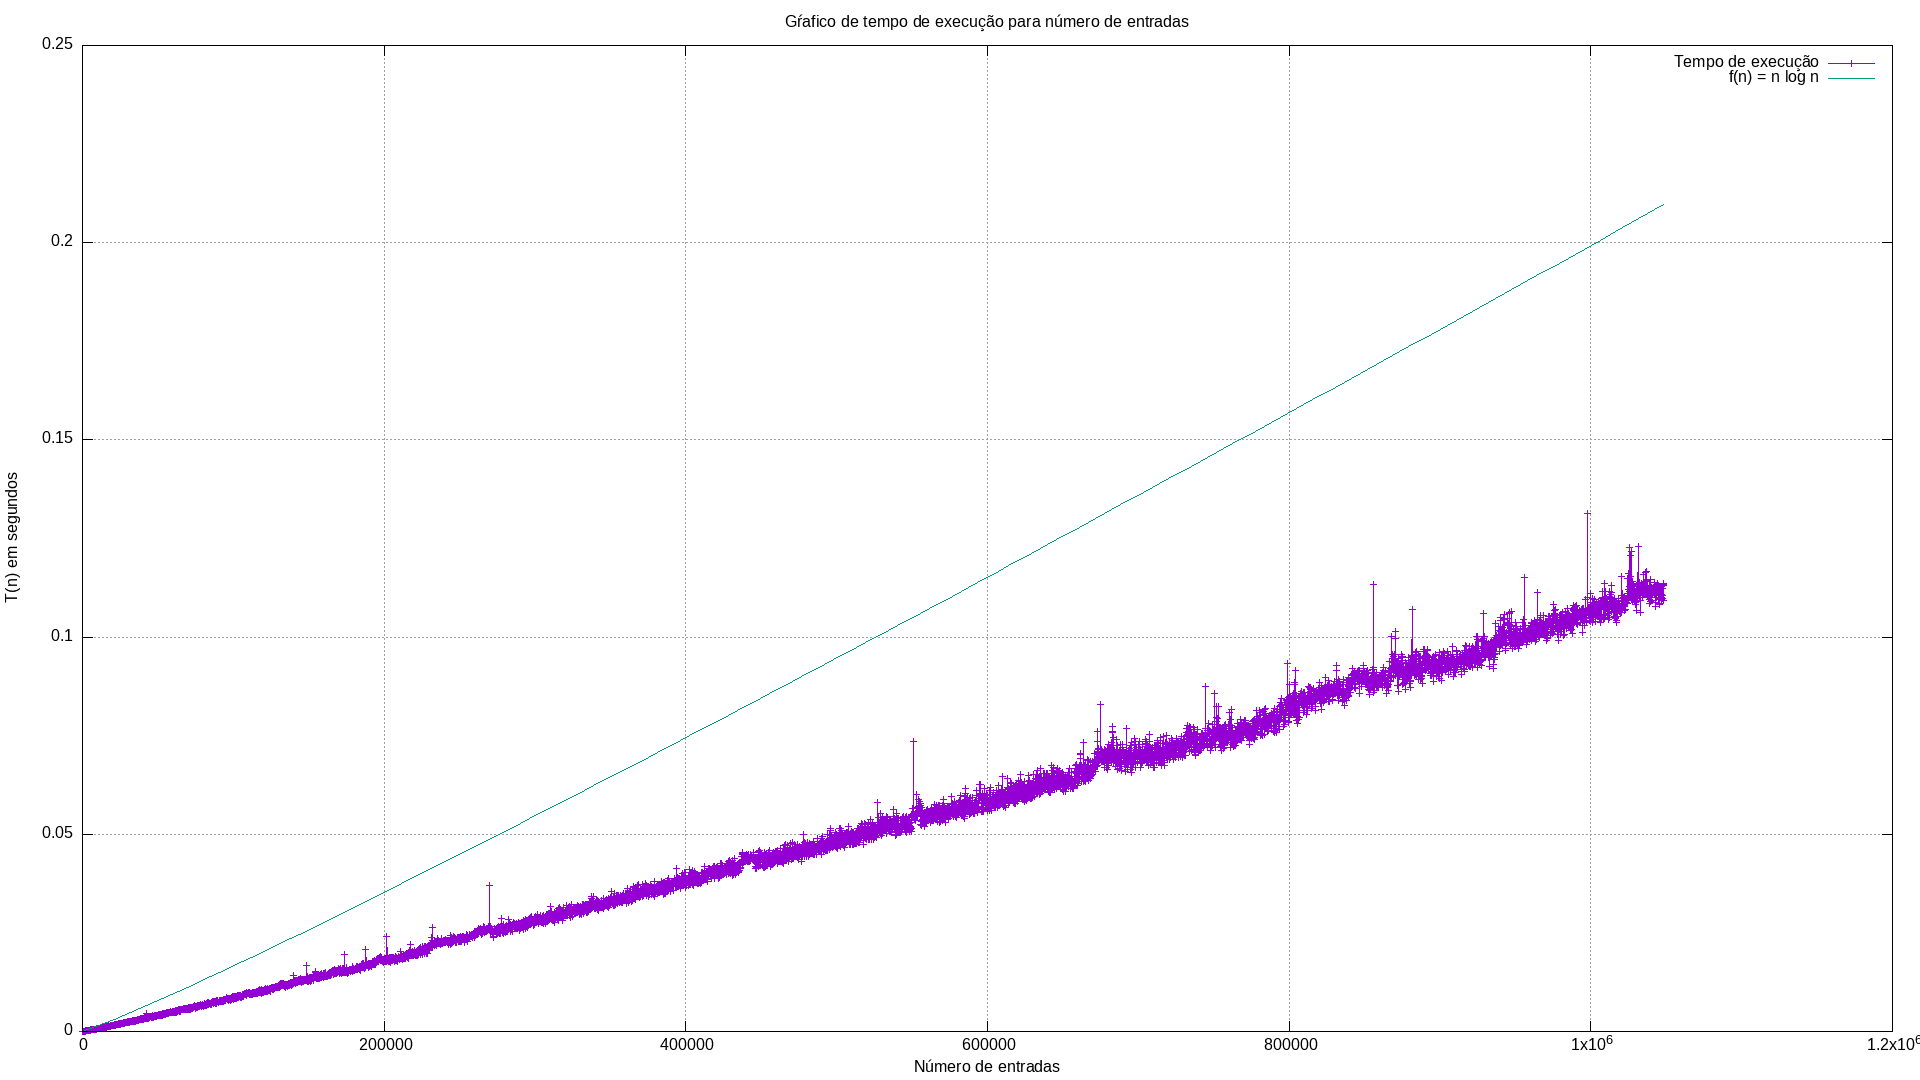
\includegraphics[width=\textwidth]{image/graphics/quickSort.png}
    \caption{Gráfico com tempo de execução do algoritmo de ordenação por particionamento}
    \label{cap:2:graph:quickSort}
\end{figure}

No gráfico \ref{cap:2:graph:quickSort}, é possível perceber que o tempo de execução do algoritmo se aproxima
da função $f(n)$ que é uma função $n \times \log n$ para $n$ com uma redução de escala para melhor percepção e comparação. Então,
utilizando como base o gráfico \ref{cap:2:graph:quickSort}, pode-se confirmar que a ordem de crescimento determinada é
precisa.

\subsection{Discussão sobre tempo de execução e uso de memória}

Sobre seu tempo de execução, o algoritmo de ordenação por particionamento é eficiente para
vetores com muitas entradas. Sobre seu uso de memória, é constante porque utiliza apenas algumas variáveis
auxiliares e transfigura o vetor origem de forma direta.

